\documentclass[12pt,fleqn]{article}\usepackage{../../common}
\begin{document}
Ekler

Seriler

Çok basit bir sonlu seri

$$ 1 + \theta + \theta^2 + ... + \theta^{n-1} $$

Üstteki toplamı daha kısa bir formülle ifade edebilir miyiz? 

$$ s_n = 1 + \theta + \theta^2 + ... + \theta^{n-1} $$

$$ \theta s_n = \theta + \theta^2 + \theta^3 + ... + \theta^n $$

Eğer 2. ifadeyi 1.'den çıkartırsak, pek çok terim iptal olacaktır,

$$ s_n - \theta s_n = 1 - \theta^n $$

$$ s_n ( 1 - \theta) = 1 - \theta^n $$

$$ s_n = \frac{1 - \theta^n}{1 - \theta} $$

Çoğunlukla fonksiyonlar sonsuz bir serinin toplamı olarak temsil
edilebilirler. Mesela ünlü üstel baz $e^x$in açılımı [8,9],

$$ e^x = 1 + x + \frac{1}{2!}x^2 + \frac{1}{3!}x^3 + ... $$

İspat

$e^x$'in özelliği nedir? Türevinin kendisine eşit olmasıdır. O zaman öyle
bir seri düşünelim ki türevini alınca kendisine eşiti olsun. Mesela

$$ 1 + x + x^2 + x^3 + ... $$

serisi ``neredeyse'' bu şarta uyuyor, çünkü türevini alınca 

$$ 0 + 1 + 2x + 3x^2 + ... $$

Bu seri, $e^x$ açılımına benzer, üstel değerler doğru, ama katsayılar
tam uymuyor. Onu telafi edebiliriz. $2x$'i $2$ ile, $3x^2$'i $3$ ile, vs
bölersek, yani $n=0,1,2,..$ için $n!$ ile bölersek, katsayılar da uyumlu
hale gelir, yani 

$$ e^x = \sum_{ n=0}^{\infty} \frac{ x^n}{n!} $$

Bir güç serisinin genel şekli

$$ f(x) = a_0 + a_1(x-x_0) + a_2(x-x_0) + ... = \sum_{ n=0}^{\infty} a_n (x-x_0)^n$$

olarak gösterilir, $a_n$ katsayıları bilinmesi gereken katsayılardır. Çoğu
durumda $x_0=0$'dir. O zaman 

$$ f(x) = \sum_{ n=0}^{\infty} a_n x_n^n = 1+x+x^2+x^3+..$$

diye gider. Herhangi bir polinom herhangi bir $c$ merkezi etrafında rahat
bir şekilde bir güç serisi (power series) olarak temsil edilebilir
(muhakkak bu serinin çoğu katsayısı sıfır değerinde olacaktır). 

Bir güç serisinin faydalı olması için sabit bir sayıya yakınsaması
(converge) gerekir. Mesela matematikteki en önemli güç serilerinden biri
olan geometrik serilere bakalım, 

$$ 1 + x + x^2 + x^3 + .. = \sum_{n=0}^{\infty} x^n  $$

Bu toplam $n \to \infty$ iken bir sayıya yaklaşır mı? 

$$ s_N = 1 + x + x^2 + ..  $$

diyelim. Şimdi bir numara, iki tarafı $x$ ile çarpalım, 

$$ x s_N = x + x^2 + x^3 + ..  $$

Eğer $s_N - xs_N$ hesaplarsak ne olur? İki üstteki formülde eşitliğin sağ
tarafından bir üsttekinin sağ tarafını çıkartırız, her iki tarafta da $x +
x^2 + x^3 + ..$ var ve bunlar iptal olur, geri kalanlar, 

$$ s_N - xs_N = 1  $$

$$ s_N(1-x) = 1 $$

$$ s_N = \frac{1}{1-x} $$

Bu seri ``başlangıcı 1, oranı $x$ olan bir geometrik seri'' olarak ta ifade
edilebilir, oran her terimin ortak katsayısı gibi görülür. Eğer başlangıç 1
oran $1-\alpha$ olsaydı,

$$ 1 + (1-\alpha) + (1-\alpha)^2 + .. $$

o zaman sonuç

$$ \frac{1}{1 - (1-\alpha)} $$

olarak çıkardı. Bu üstteki yöntemle kontrol edilebilir. Yani sonuç için
başlangıç değeri bölünene, oran denilen değer ise 1'den çıkartılıp
bölünene yazılır.

Bir diğer seri

$$ 1 - x + x^2 - x^3 + .. $$

güç serisi neye yaklaşır? 

Yine aynı numara, ama bu sefer $-x$ ile çarpalım,

$$ s_N  = 1 - x + x^2 - x^3 + .. $$

$$ -x s_N = -x + x^2 - x^3 + .. $$

1. formülden 2.'yi çıkartalım, 

$$ s_N + x s_N = 1$$

$$ (x+1)s_N  = 1$$

$$ s_N  = \frac{1}{x+1} $$

\newpage

Türev Alırken Bölüm Kuralı (Quotient Rule)

Bölüm kuralı şöyle gösterilir 

$$ \frac{ u(x)}{v(x)} = \frac{u(x)'v(x) - u(x)v(x)'}{v(x)^2} $$

Ya da $x$ göstermeden

$$ \frac{ u}{v} = \frac{u'v - uv'}{v^2} $$

Bu formülü hatırlamak biraz zor gelebilir. Eğer hatırlamıyorsak hatırlaması
daha basit olan Çarpım Kuralı (product rüle) üzerinden
türetebiliriz. Çarpım kuralı bildiğimiz gibi

$$ (uv)' = u'v + uv' $$

Burada bir numara yaparak 

$$ (u \ \frac{ 1}{v})' $$

üzerinde Carpım Kuralını kullanarak türev alacağız, böylece otomatik olarak
arka planda aslında $u/v$'nin türevini aldırtmış olacağız. 

$$ \bigg(u \ \frac{ 1}{v}\bigg)' = 
u \bigg(\frac{1}{v}\bigg)' + u' \bigg(\frac{1}{v}\bigg)
$$

Bu arada

$$ \bigg(\frac{ 1}{v}\bigg)'  = -\frac{v'}{v^2} $$

Bölümde $v'$ var, çünkü unutmayalım $v$ aslında $v(x)$, o zaman ana
formülde yerine koyalım

$$  = 
-u\frac{v'}{v^2}  + u' \bigg(\frac{1}{v}\bigg)
$$

$$  = 
\frac{u' }{v} -\frac{uv'}{v^2}
$$


Birinci terimde bölüm ve böleni $v$ ile çarpalım, ki iki terimi
birleştirebilelim, 

$$  = 
\frac{u'v }{v^2} -\frac{uv'}{v^2} = 
\frac{u'v-uv'}{v^2}
$$

\newpage

Bazı $e$, Log Özellikleri

Bazen $\log$ bazen $\ln$ kullanıldığını görürsünüz. Eğer $\ln$
kullanılırsa bu $\log$ ifadesinin $e$ baz kullanan hali demektir, yani
$\log_e$. 

Çarpım log'u, logların toplamı olur.

$$ \log xy = \log x + \log y $$

Bölüm log'u, logların çıkartılması olur.

$$ \log x/y = \log x - \log y  
\mlabel{1}
$$

Aynı baz kullanan çarpımlar, tek baza indirilip üstleri toplanabilir.

$$ e^a \cdot e^b = e^{a+b} $$

Üstü olan bir ifadenin log'u, üst değerini aşağı indirir.

$$ \log(x^y) = y \log(x) $$

Üstün üstü (son üst tüm bazı kapsayacak şekilde ise) direk üstlerin
çarpımına çevirilebilir.

$$ (e^x)^y = e^{xy} $$

$\ln$'nin bazı $e$ olduğuna göre, $e$ üzeri $\ln$ birbirini iptal eder,
yani

$$ x = e^{\ln x} $$

Bu ifade (1)'den türetilebilir ama yine de ayrı vermek iyi olur, $1/x$'in
log'u $x$'in negatifini verir. 

$$ \log(1/x) = -\log(x) $$

\newpage

Kısmi Kesirler Yöntemi (Partial Fractions Method)

Bazen şu şekildeki bir kesiri 

$$ \frac{8x + 22}{(x-1)(x+5)} $$

bölendeki her çarpan ayrı bir kesir parçasında olacak şekilde o parçaların
toplamı olarak göstermek faydalıdır. 

$$ \frac{...}{(x-1)} + \frac{...}{(x+5)} $$

Bu tür bir parçalı kesirin verisini almak çok daha kolaydır
mesela. Fakat bu parçalama işlemini nasıl yapacağız?

Cebir kullanarak bu problemi çözebiliriz. Üstte nokta nokta olan yerlerin
ne olduğunu merak ediyoruz, o zaman onlara $A,B$ değişkenlerini atarsak

$$ \frac{A}{(x-1)} + \frac{B}{(x+5)} = \frac{8x + 22}{(x-1)(x+5)}$$

Eğer bölüm kısmında temiz bir eşitlik elde etmek istiyorsak, o zaman
üstteki kesirlerin bölen kısmını birbirinin aynısı haline getirmeliyiz. İlk
terimin bölüm, bölen kısmını $(x+5)$, ikincisinin bölüm, bölen kısmını
$(x-1)$ ile çarparsak, bu eşitliği elde ederiz. 

$$ \frac{(x+5)A}{(x-1)(x+5)} + \frac{(x-1)B}{(x+5)(x-1)} = 
\frac{8x + 22}{(x-1)(x+5)}
$$

Bölen kısmı birbirine eşit olduğuna göre, artık sadece kesirlerin üst
kısmını kullanabiliriz, çünkü aradığımız bilinmeyenler orada. 

$$ (x+5)A + (x-1)B = 8x+22 $$

Eşitliğin sol tarafının açılımını düşünürsek, 

$$ xA + .. + Bx + .. = 8x + .. $$

$$ x(A + B) +  .. = 8x + .. $$

ve her iki tarafta $x$'in katsayılarının aynı olması zorunluluğundan
hareketle

$$ A + B = 8 $$

olacaktır. Benzer şekilde geri kalan sabitleri eşitlersek 

$$ 5A - B = 22 $$

O zaman elimizde iki bilinmeyen, iki denklem var, bu sistemi çözmek çok
kolay! 

$$ B = 5A - 22 $$

Öteki denkleme sokalım

$$ A + 5A - 22 = 8 $$

$$ 6A = 30 $$

$$ A = 5 $$

$$ B = 3 $$

Demek ki kısmi kesirlerimiz şöyle olacak 

$$ \frac{5}{(x-1)} + \frac{3}{(x+5)} = \frac{8x + 22}{(x-1)(x+5)}$$

\newpage

Trigonometri

Basit bazı temel bilgilerin üzerinden geçelim. Sinüs, kosinüs, tanjant nedir?
Karşı, komşu, hipotenüs kullanan bazı tanımlar akılda kalmış olabilir, mesela
alttaki açı $\alpha$ ve dik üçgenler için, karşı bölü hipotenüs sinüs, komşu
bölü hipotenüs kosinüs, karşı bölü komşu tanjant.

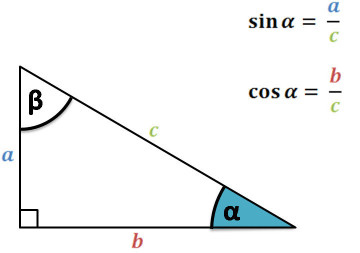
\includegraphics[width=20em]{trig-reciprocal2.jpg}

Aslında tanjant'ın esas tanımı sinüs bölü kosinüs,

$$
\tan \alpha = \frac{\sin\alpha}{\cos\alpha} = \frac{a / c}{b / c} = \frac{a}{b}
$$

bölen $c$ iptal olduğu için geri kalanlar karşı bölü komşu. 

Pitagor Kanunu

$a^2 + b^2 = c^2$

İspat

Dik üçgenimizi alıp yanyana koyarak bir kare oluşturuyoruz, artık hem dış
çeperde bir kare var, ayrıca iç kısımda da bir kare var. 

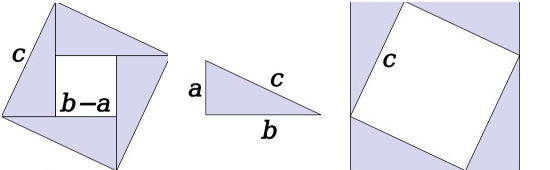
\includegraphics[width=20em]{Pythagoras.png}

Bu karenin kenarları $b-a$ büyüklüğünde, alanı tabii ki $(b-a)^2$. Büyük karenin
alanı $c^2$. Ama eğer büyük karenin alanını görülen beş tane parçayı toplayarak
elde edebilirsek, Pitagor formülüne erisebiliriz.

$$
(b-a)^2 + 4 \frac{ab}{2} = (b-a)^2 + 2 ab = b^2 -2ab + a^2 + 2ab = a^2 + b^2
$$

Büyük kare eşitliğinden bu alan $c^2$'dir demiştik, o zaman

$$
c^2 = a^2 + b^2
$$

İspatı tamamlamış olduk.

Şimdi Pitagor kullanarak önemli bir trigonometrik eşitlik elde edeceğiz, alttaki
dik üçgeni oluşturursak, $\theta$ ne olursa olsun mavi renkli çemberin yarıçapı,
ve dik üçgenin hipotenüsü 1 olacaktır, ve $\sin\theta = a / 1$ olduğu için
$\sin\theta = a$, yani karşı kenar $\sin\theta$, komşu kenar $\cos\theta$.

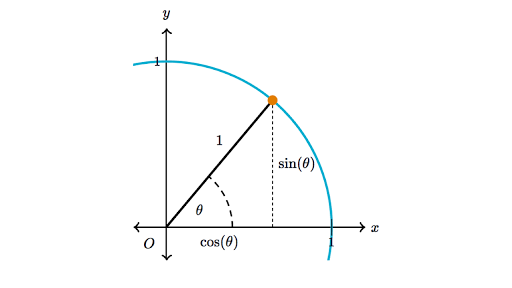
\includegraphics[width=20em]{PythagorSinCos.png}

Bu kenar bilgilerine Pitagor üzerinden

$$
a^2 + b^2 = 1^2 
$$

$a,b$ yerine koyarsak,

$$
\cos^2\theta + \sin^2\theta = 1
$$

Bu önemli bir trigonometrik eşitliktir.

Diğer Trigonometrik Eşitlikler

Toplam Formülleri

Acı toplama eşitliklerine bakalım. Bu eşitlikler

$$
\cos(A+B) = \cos A \cos B - \sin A \sin B
$$

$$
\sin(A+B) = \sin A \cos B + \cos A \sin B
$$

Ispata gelelim. Önce Euler eşitliği,

$$
e^{i\theta} = \cos\theta + i\sin\theta
$$

Şimdi diyelim ki $\theta = A+B$, o zaman [11],

$$
\cos(A+B) + i\sin(A+B) = e^i(A+B)
$$

$$
= e^{iA} \cdot e^{iB}
$$

$$
= (\cos A + i\sin A) (\cos B + i\sin B)
$$

Çarpımı açarsak,

$$
= \cos A \cos B + i\cos A \sin B +
i\sin A \cos B - \sin A \sin B
$$

Dikkat son terimdeki eksi işaretin sebebi $i \cdot i = -1$ olması çünkü hayali
sayı $i$'nin tanımı $i = \sqrt{-1}$. 

Bir gruplama yapalım, 

$$
= \cos A \cos B - \sin A \sin B + i (\cos A \sin B + \sin A \cos B )
$$

Buraya nereden geldiğimizi hatırlayalım, üstteki ifadenin $\cos(A+B) + i\sin(A+B)$'e
eşit olması gerekir. Eşitlik ne demektir? Üstteki formülün reel kısmını
$\cos(A+B) + i\sin(A+B)$'in reel kısmına, hayali kısmının yine aynı formülün
hayali kısmı ile eşit olması demektir. O zaman ispat tamamlanmış oldu.

Çift Açı Formülleri

İspatladığımız

$$
\cos(A+B) = \cos A \cos B - \sin A \sin B
$$

formülünde eğer $B$ yerine $A$ kullanırsak, o zaman $2A$ elde ederiz, bunun
açılımı neye eşit olur?

$$
\cos(A+B) = \cos(A+A) = \cos(2A) = \cos A \cos A - \sin A \sin A
$$

$$
\cos(2A) = \cos A^2 - \sin A^2
$$

Ayni teknigi $\sin(A+B)$ uzerinde uygularsak,

$$
\sin(A+B) = \sin(A+A) = \sin(2A) =
\sin A \cos A + \cos A \sin A
$$

Bu iki terim birbirinin aynısı, o zaman

$$
\sin(2A) = 2\sin A \cos A
$$

Şimdiye kadar elde ettiğimiz

$$
\cos^2\theta + \sin^2\theta = 1, \quad
\cos^2\theta - \sin^2\theta = \cos2\theta
$$

formüllerinden ek eşitlikler türetmek mümkün. Eğer iki formülü toplarsak

$$
2\cos^2\theta = 1 + \cos2\theta 
$$

eğer 2'inciyi 1'inciden çıkartırsak,

$$
2\sin^2\theta = 1 - \cos2\theta
$$

elde ederiz.

Küçük Açı Yaklaşıklaması (Small Angle Approximation)

Bazı fizik kitaplarında ve eğer ufak açılar sözkonusu ise bazen $\sin\theta
\approx \theta$ geçişi yapıldığını görüyoruz. Bu nereden geliyor?

Sinüs fonksiyonu üzerinde Maclaurin açılımı [4] yaparsak (yani sıfır etrafında
Taylor açılımı),

$$
\sin\theta =
\theta -
\frac{\theta^3}{3!} +
\frac{\theta^5}{5!} -
\frac{\theta^7}{7!} + ...
$$

Radyan olarak düşünürsek eğer $\theta$ çok küçük, yani sıfıra yakın ise küpü
alınan çok küçük değer daha da küçülecektir, o zaman ikinci terim dahil olmak
üzere tüm diğer terimler yok sayılabilir,

$$
\sin\theta \approx \theta
$$

Dahası da var! Çok ufak bir açının kosinüsü 1'e yakındır, ve tanjant sinüs bölü
kosinüs olduğu için bölen 1 iptal edilir, geriye kalanlar,

$$
\tan\theta \approx \sin\theta \approx \theta
$$

Faydalı olabilir!

Sayısal olarak kontrol edelim,

\begin{minted}[fontsize=\footnotesize]{python}
theta = 0.01
print (np.sin(theta))
print (np.tan(theta))
\end{minted}

\begin{verbatim}
0.009999833334166664
0.010000333346667207
\end{verbatim}

Üstteki numaralar bazen ilginç şekillerde karşımıza çıkabilir, mesela bir
eğrinin eğiminin ne olduğunu hatırlarsak,

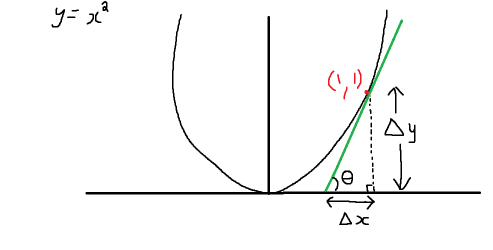
\includegraphics[width=20em]{slope_tan2.png}

Eğim $\Delta y / \Delta x$, ki bu yaklaşık olarak türevin ta kendisi değil
midir, yani $dy / dx$? Evet. Aynı şekilde üstte gördüklerimizden hareketle
bu eğime $\tan\theta$ diyebiliriz, ve ufak açılar sözkonusu ise
$\tan\theta \approx \theta \approx dy / dx$!

Ters Trigonometrik Formüller (Inverse Trigonometric Functions)

$\cos x$ için $\cos^{-1} x$ ya da $\arccos x$ ile gösterilen ters
trigonometrik formüldür. $\sin x$ ve $\tan x$ için aynı şekilde. 

Bu ters fonksiyonların türevi nasıl alınır? $\theta = \tan^{-1}x$ örneğinde
görelim. Elde etmek istediğimiz $d\theta/dx$. 

Eğer

$$ \tan^{-1}x = \theta$$

ise, o zaman 

$$ \tan\theta = x $$

$x$'i aslında $\theta$'ya bağlı bir $x(\theta)$ fonksiyonu olarak görebiliriz. 
Eğer iki tarafın $\theta$'ya göre türevini alırsak

$$ \frac{dx}{d\theta} = \sec^{2}\theta $$

Bizim istediğimiz bunun tersi, o zaman bölümü tersine çevirelim

$$ \frac{d\theta}{dx} = \frac{1}{\sec^{2}\theta} $$

Pitagor Eşitliklerinden bildiğimize göre

$$ \sec^{2}\theta = \tan^{2}\theta + 1 $$

Yerine geçirelim

$$ \frac{d\theta}{dx} = \frac{1}{\tan^{2}\theta + 1} $$

İlk başta tanımladığımıza göre $\tan\theta = x$, bunu da üstte yerine
koyalım

$$  = \frac{1}{x^2 + 1} $$

\newpage

İçiçe Fonksiyonlar (Composite Functions) [1, sf. 191, 227]

$$ y = \frac{3}{2}x = \frac{1}{2}3x $$

bir içiçe fonksiyon olarak görülebilir. 

$$ y = \frac{1}{2}u, \ u=3x $$

dersek, $y$ içindeki $u$ bir başka fonksiyon olabilir. Yani aslında 

$$ y = f(u) $$

$$ u = g(x) $$

Yani

$$ y = f(g(x)) $$

Üstteki form bazen 

$$ y = f \circ g $$

olarak ta gösterilebiliyor. 

\newpage

Zincirleme Kanunu (İçiçe Fonksiyonlar İçin)

Eğer $f(u)$, $u=g(x)$ noktasında, ve $g(x)$, $x$ noktasında türevi
alınabilir durumda ise, o zaman içiçe fonksiyon $(f \circ g)(x) = f(g(x))$
$x$ noktasında türevi alınabilir demektir, ve

$$ (f \circ g)'(x) = f'(g(x)) \cdot g'(x) $$

doğru olacaktır. Leibniz notasyonu ile 

$$ \frac{ dy}{dx} = \frac{ dy}{du} \cdot \frac{ du}{dx} $$

Üstteki formülü kesirlerin çarpımı olarak görmek kısmen doğru olabilir, en
azından hatırlamak için iyi, ama formel ispat başka şekilde yapılıyor,
detaylar için ``$dy/dx$ bir kesir olarak görülebilir mi?'' yazısına
bakabilirsiniz.

Türev alırken $'$ işaretinin kullanılabilme sebebi fonksiyonda tek değişken
olduğu zaman neye göre türev alındığının bariz olması.

Örnek 

Başta verilen örnek için $dy/dx$' i bulun. 

$$ \frac{ dy}{dx} = \frac{ 3}{2}, \
\frac{dy}{du} = \frac{ 1}{2}, \
\frac{ du}{dx} = 3
 $$

$$ \frac{ dy}{dx} = \frac{ dy}{du} \cdot \frac{ du}{dx} $$

O zaman 

$$ \frac{ 1}{2} \cdot 3 = \frac{ 3}{2} $$

\newpage

Parçalı Entegral (Integration by Parts)

Aslında parçalı entegral türevlerin çarpım kuralının bir uzantısı sadece
[12, sf. 17]. 

$$
\frac{\ud }{\ud x} [u v] = \frac{\ud u}{\ud x} v + u \frac{\ud v}{\ud x}
$$

Şimdi iki tarafın türevini alalım,

$$
\int_{a}^{b} \frac{\ud}{\ud x} [u v] \ud x =
\int_{a}^{b} \frac{\ud u}{\ud x} v \ud x +
\int_{a}^{b} u \frac{\ud v}{\ud x} \ud x 
$$

Ustteki temel Calculus kanunundan geliyor,

$$
\Rightarrow u v |_{a}^{b} =
\int_{a}^{b} \frac{\ud u}{\ud x} v \ud x + 
\int_{a}^{b} u \frac{\ud v}{\ud x} \ud x 
$$


$$
\Rightarrow \int_{a}^{b} u \frac{\ud v}{\ud x} =
u v |_{a}^{b}  -
\int_{a}^{b} \frac{\ud u}{\ud x} v \ud x
$$

Bu parçalı entegral formülüdür. Daha rahat hatırlamak için çoğu zaman
$u=f(x),v=g(x)$ kabul edilir, o zaman $du = f'(x)dx$ ve $dv = g'(x)dx$
olur, ve şu form ortaya çıkar,

$$ \int u \ud v = uv - \int v \ud u$$

Bu formül birinci entegral $\int u \ud v$'yi ikinci bir entegral $\int v \ud u$
üzerinden tarif etmiş olur, bazı durumlarda ikinci entegral hesabı daha kolay
olabileceği için o tercih edilebilir, ve parçalı entegral formülüyle o entegrale
geçiş yapılmış olur [1, sf. 562].

\newpage

Eşsizlikler (Singularities) 

Eşsiz nokta bir fonksiyonun analitikliği kaybettiği yerdir. Sıfır ile
bölünmek mesela eşsizlik sebeplerinden bir tanesidir. Ya da içinde dallanma
noktası taşıyan tüm fonksiyonlar o noktada analitikliği kaybederler,
türevleri alınamaz, bu sebeple eşsizlik taşırlar. Mesela $f(z) = z^{1/2}$
ya da $f(z) = \sqrt{z}$ fonksiyonunda, her $z$ değeri için iki tane
$z^{1/2}$ değeri vardır.

Basit örnek, 

$$ f(z) = \frac{ \sin z}{z} $$

Bu fonksiyon $z=0$ noktasında tanımsızdır, çünkü $f(0) = 0/0$ ve sıfır ile
bölmek tanımsızdır, o zaman $f(z)$ sonlu hayali düzlemin her yerinde
analitiktir, sadece $z=0$ noktasında değildir [5, sf 364]. 

Şimdi ilginç bir numara, bazen eşsizliği ``çıkartmak'' mümkündür; önce suna
dikkat, $z \to 0$ iken fonksiyonun limiti var,
$$ \lim_{z \to 0} \frac{ \sin z}{z} = \lim_{z \to 0} \frac{\cos z}{1} = 1 $$


Üstteki $\cos z/1$ geçişini yapabildik çünkü L'Hospital kuralını hatırlarsak
$\lim_{z \to z_0} f(z)/g(z) = \lim_{z \to z_0} f'(z)/g'(z)$. O zaman parçalı bir
fonksiyon yaratarak eşsiz noktadaki ``boşluğu doldurmak'' mümkündür, yani bu
fonksiyonu her noktasında türevi alınır hale getirebiliriz. Fonksiyon $f(z)$'yi
``sarmalayan'' yeni bir $f(z)$ yaratırsak,

$$ 
g(z) = \left\{ \begin{array}{ll}
\frac{\sin z}{z} & z \ne 0 \\
1 & z = 0
\end{array} \right.
 $$

Bu fonksiyonun $z=0$ noktasında artık türevi alınabilir. Kontrol edelim, 

$$ f'(0) = \lim_{z \to 0} \frac{f(0)-f(z)}{z}  $$

$$ = \lim_{z \to 0} \frac{1-\sin(z)/z}{z} $$

$$ = \lim_{z \to 0} \frac{z-\sin(z)}{z^2} $$

L'Hospital,

$$ = \lim_{z \to 0} \frac{1 - \cos z}{2z} $$

Tekrar

$$ = \lim_{z \to 0} \frac{ \sin(z)}{2} $$

$$ = 0 $$

$z=0$ noktasına {\em çıkartılabilen eşsizlik} ismi verilir, çünkü
fonksiyonun eşsizlik noktasındaki değerini o noktadaki limiti haline
getirirsek, o noktadaki eşsizliği çıkartmış oluruz. 

\newpage

$dy/dx$ bir kesir olarak görülebilir mi? 

Mesela [1, sf. 225] bölüm 3.8'te türev $dy/dx$'in bir kesir, bir oran
olmadığı söylenir. Fakat bu şekilde görülemez mi? Çünkü $dy = f'(x)dx$
formülünde $dx$ için gerçek sayılar verip sonucu (diferansiyeli) $dy$
olarak hesaplayabiliyoruz. Eğer bu formülü tekrar düzenlersek $dy/dx$ for
kesir olarak görülebilirdi.. belki.

Fakat bu teorik olarak tamamiyle, her zaman işlemiyor. Yani pratikte bazen
bu şekilde görebiliyoruz, fakat işin en temelinde durum böyle değil.

Tarihsel olarak, Calculus'u keşfeden matematikçi Leibniz bu notasyonu ileri
sürdüğünde $dy/dx$'i bir kesir olarak düşünmüştü, bu değerin temsil ettiği
büyüklük ``$x$'deki sonsuz ufak (infinitesimal) değişimin $y$'de yarattığı
sonsuz ufak değişime oranı'' olarak düşünülüyordu.

Fakat Calculus'un sonsuz ufaklıklar mantığını reel sayılar çerçevesinde
kullanmak teorik olarak pek çok problemi beraberinde getiriyor. Bunlardan
biri, sonsuz ufaklığın reel sayıların olduğu bir çerçevede var
olamamasıdır! Reel sayılar önemli bir önşartı yerine getirirler, bu şartın
ismi Arşimet Şartı'dır. Bu şarta göre, ne kadar küçük olursa olsun herhangi
bir pozitif tam sayı $\epsilon > 0$, ne kadar büyük olursa olsun reel bir
sayı $M>0$ bağlamında, $n\epsilon > M$ şartını doğrulayacak bir doğal sayı
$n$ her zaman mevcuttur. Fakat sonsuz ufak bir $\xi$ o kadar ufak olmalıdır
ki onu kendisine ne kadar eklersek ekleyelim, hiçbir zaman 1'e erişemeyiz,
ki bu durum Arşimet Şartına aykırı olur [..]

Bu problemlerden kurtulmak için takip eden 200 sene içinde Calculus ta
temelinden başlayarak sıfırdan tekrar yazılmıştır, ve şimdi gördüklerimiz
bu sıfırdan inşanın sonuçları (mesela limit kavramı bunun bir sonucu). Bu
tekrar yazım sayesinde / yüzünden türevler artık bir oran değil, bir limit.

$$ \lim_{h \to 0} \frac{f(x+h) - f(x)}{h}$$

Bu ``oranın limiti''ni ``limitlerin oranı'' olarak yazamayacağımız için
(çünkü hem bölüm, hem bölen sıfıra gidiyorlar), o zaman türev bir oran
değildir.

Fakat Leibniz'in notasyonu o tür kullanımı özendiriyor sanki, oraya doğru bir
çekim yaratıyor, hatta bazen notasyonu o şekilde görmenin işe yaradığı bile
oluyor, yani çoğu zaman bu notasyon sanki kesirmiş {\em gibi}
davranıyor. Zincirleme Kanunu mesela

$$ \frac{dy}{dx} = \frac{dy}{du}\frac{du}{dx} $$

Türevlerin kesir olarak görüldüğü bir durumda üstteki ifade hakikaten doğal
duruyor. Ya da Tersi Fonksiyon (Inverse Function) teorisi

$$ \frac{dx}{dy} = \frac{1}{\frac{dy}{dx}} $$

sonucu da eğer türevleri kesir olarak düşünüldüğü bir ortamda doğal
gelecektir. İşte bu sebeple, yani notasyonun çok güzel ve özendirdiğinin
çoğunlukla doğru şeyler olması sebebiyle artık bir limiti temsil eden
notasyonu kullanmaya devam ediyoruz, her ne kadar artık gerçekten bir
kesiri temsil etmiyor olsa bile. Hatta şu ilginç tarihi anektodu ekleyelim,
bu notasyon o kadar iyidir, Newton'un notasyonu olan tek tırnak ($y'$ gibi)
işaretinden o kadar ileridir ki bazılarının iddiasına göre İngiltere'deki
matematik ve bilim kara Avrupa'sının yüzyıllarca gerisinde kalmıştır -
çünkü Newton ve Leibniz arasında Calculus'u kimin keşfettiği konusunda bir
çatışma yaşandı (bugünkü konsensüs ikisinin de Calculus'u aynı anda
keşfettiği üzerine), ve bu çatışma ortamında İngiliz bilim çevresinin
Avrupa'daki ilerlemeleri, Leibniz notasyonunu dışlayıp Newton'u takip
etmeleri sonucunu getirdi.. ve bu sebeple pek çok alanda geri kaldılar
[..].

Sonuca gelirsek, $dy/dx$'i bir kesir gibi yazıyor, ve pek çok hesapta onu
sanki bir kesirmiş gibi kullanıyor, kullanabiliyor olsak bile, $dy/dx$ bir
kesir değildir, sadece filmerde o rolü oynar (!).

\newpage 

Sonsuz Kuvvet, Calculus'un Temeli

Calculus'un bu kadar başarılı olmasının sebebi nedir? Calculus'un
başarısının altında yatan sır çetrefil problemleri ufak parçalara
bölebilmesi [10]. Tabii ki bir problemi parçalara bölmeyi pek çok diğer
alanda da görüyoruz. Ama Calculus bunu en radikal şekilde yapıyor,
problemleri {\em sonsuz ufak parçalara} bölebiliyor. Bir problemi bir, iki,
vs. parçaya bölmek yerine onu bölüyor, bölüyor, ta ki problem unufak sonsuz
tane parçalar haline gelinceye dek, sonra problemi o ufacık parçalar için
çözüyor, ki bu noktada çoğunlukla çözüm büyük problemden çok daha rahattır.
Sonra herşeyi biraraya koyuyor, bu adım bölmekten daha zor olabilir ama
yine de esas büyük problemi çözmekten daha kolaydır, ve çözüme ulaşılıyor.

Yani Calculus iki adımda işini yapıyor, bölmek ve biraraya koymak. Bölme
kısmına diferansiyel Calculus deniyor, biraya koyma kısmına entegral
Calculus.

Calculus aslında çok eskidir, çünkü biraz önce bahsettiğimiz prensibin
takip edilmesi için muhakkak formülsel formlar takip etmek şart
değil. Mesela M.Ö. 250 zamanında yaşamış Arşimet bir çemberin alanını aşağı
yukarı şöyle bir yaklaşımla buldu. Elimizde bir daire var, bir pizza
diyelim, bu pizzanın alanını bulmak istiyoruz,

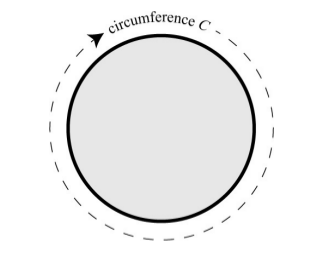
\includegraphics[height=4cm]{circ_1.png}

Bildiklerimiz pizzanın yarıçapı (radıus) $r$ ve çevresi $C$. Eğer pizzadan
ufak bir parça kessek parçanın iki yanı tabii ki $r$ olur.

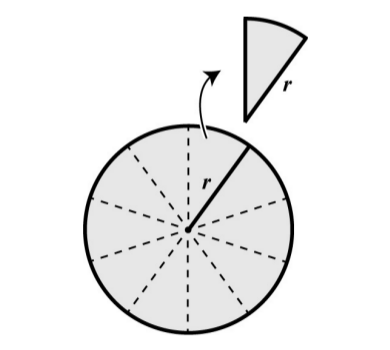
\includegraphics[height=5cm]{circ_2.png}

Alan hesabı yapmak istiyoruz, bir fikir şu, pizzayı dört parçaya bölelim,
sonra parçaları yanyana koyalım.

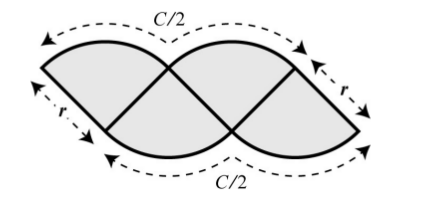
\includegraphics[height=3cm]{circ_3.png}

Bu pek düzgün bir şekil olmadı, alanı rahatça hesaplamak kolay değil. Emin
olduğumuz bir şey var, engebeli olsa da üst kısım $C/2$ uzunluğunda, alt
kısım aynı şekilde. Bir dikdörtgen olsa iyi olurdu, o şekle erişmemiş
olmamızın sebebi yeterince ufak parçaya bölmemiş olmamız mı acaba? 8
parçaya bölelim, ve yine parçaları yanyana koyalım,

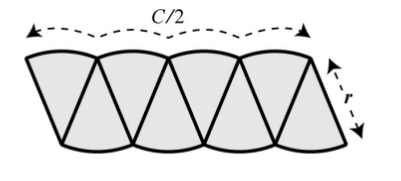
\includegraphics[height=3cm]{circ_4.png}

Bu şekil bir paralelogramı andırmaya başladı. Fena değil, üst, alttaki
sınırların engebesi azaldı, düzleşmeye başladılar. Aslında bir
dikdörtgenimsi sekle ufak bir hamle ile daha yaklaşabiliriz, soldaki
parçanın yarısını alıp sağ tarafa yapıştıralım,

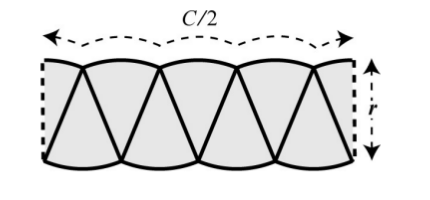
\includegraphics[height=3cm]{circ_5.png}

Güzel. Hala tam düzleşme elde edemedik, eh ama şimdiye kadar ufalta ufalta
bayağı yol aldık, daha da ufaltalım, 16 parça,

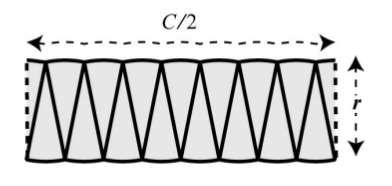
\includegraphics[height=3cm]{circ_6.png}

Ne kadar parçaya bölersek o kadar dikdörtgene yaklaşıyoruz. Üstteki şekil
dikdörtgene yaklaştığı için sonsuz parçanın birleşmesinin limite giderken
tam bir dikdörtgen olacağını biliyoruz. 

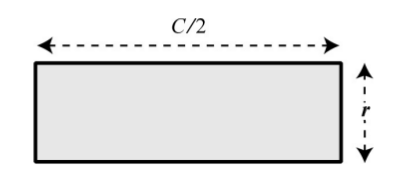
\includegraphics[height=3cm]{circ_7.png}

Bu dikdörtgenin alanını bulmak çok kolay, $r \cdot C/2$. Eh bölünen parçaları
kaybetmedik, hepsini kullandık, o zaman bu alan en baştaki dairenin de alanı
olmalı! Arşimet işte daire alanını, matematiksel ispatı ile beraber, işte böyle
hesapladı

Not: Formülleri daha detaylandırırsak, $C$'nin $r$ ile ilişkisi zaten
biliniyorsa, $C = 2 \pi r$, buradan alan

$$
A = r C/2 = r (2 \pi r)/2 = \pi r^2 
$$

Fakat $C$ bazlı alan ispatının en dahiyane kısmı sonsuzluğun kullanılma
şekli. 4, 8, 16 ile başladık, parçaların toplamı gitgide daha çok dikdörtgene
benzemeye başladı. Ama sonsuz tane parçanın limitinin ortaya çıkarttığı şekil
tam dikdörtgen olacaktı, ve nihai hesapta bu formu kullanabilirdik. İşte
Calculus'un temeli burada yatıyor. Sonsuzluğa gidince herşey daha basit hale
geliyor.


\newpage

Bazı yaygın z-transform'ları 

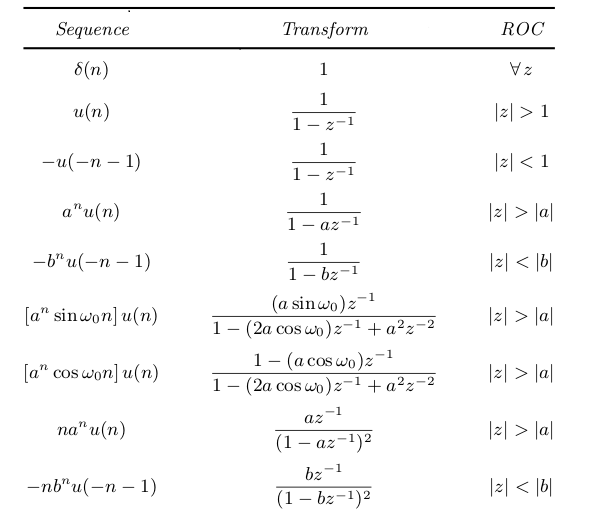
\includegraphics[height=12cm]{z_01.png}

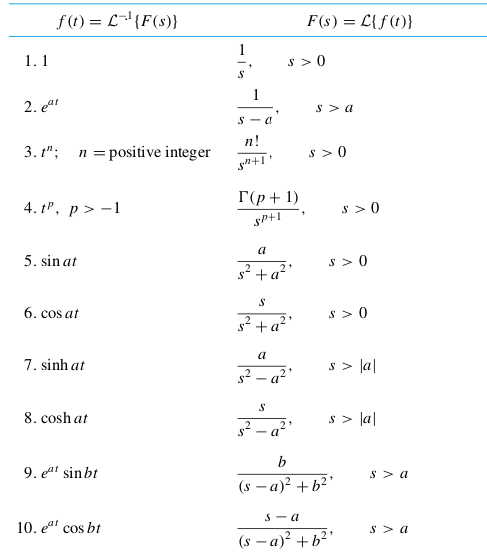
\includegraphics[height=12cm]{lap_1.png}

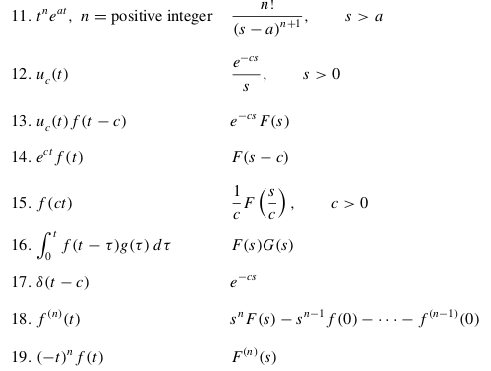
\includegraphics[height=9cm]{lap_2.png}

Kaynaklar 

[1] Thomas, {\em Thomas Calculus, 11th Edition}

[2] Ifeachor, {\em Digital Signal Processing}, pg. 105

[3] Slicer, {\em Digital Signal Processing using Matlab}, pg. 119

[4] Wikipedia, {\em Small angle approximation},
    \url{https://en.wikipedia.org/wiki/Small-angle_approximation}

[5] B. A. Shenoi, {\em Introduction to DSP and Filter Design}, pg. 41

[6] Mauch, {\em Introduction to Methods of Applied Mathematics}

[7] Mattuck, {\em Introduction to Analysis}

[8] Wikipedia, {\em Power Series}, \url{http://en.wikipedia.org/wiki/Power_series}

[9] Moore, {\em Introduction to Partial Differential Equations}

[10] Strogatz, {\em Infinite Powers}

[11] Blackpenredpen, {\em Angle Sum formula, proof by complex number},
     \url{https://www.youtube.com/watch?v=OcXqF8l2crI}

[12] Gockenbach, {\em Understanding and Implementing FEM}

\end{document}


